% Created by tikzDevice version 0.10.1 on 2018-06-07 09:38:33
% !TEX encoding = UTF-8 Unicode
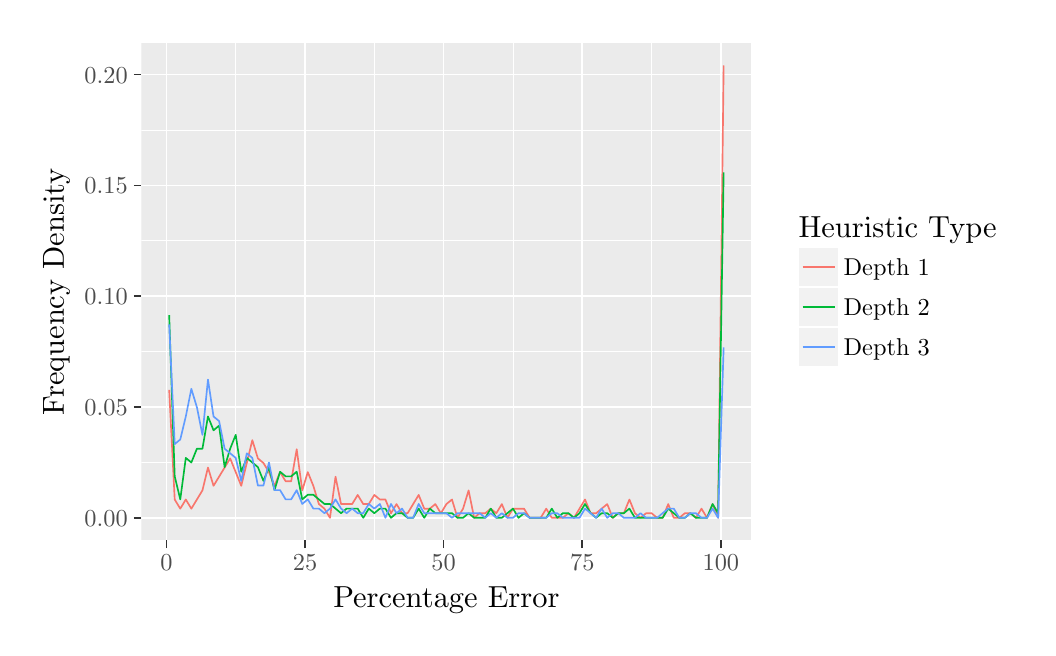
\begin{tikzpicture}[x=1pt,y=1pt]
\definecolor{fillColor}{RGB}{255,255,255}
\path[use as bounding box,fill=fillColor,fill opacity=0.00] (0,0) rectangle (361.35,216.81);
\begin{scope}
\path[clip] (  0.00,  0.00) rectangle (361.35,216.81);
\definecolor{drawColor}{RGB}{255,255,255}
\definecolor{fillColor}{RGB}{255,255,255}

\path[draw=drawColor,line width= 0.6pt,line join=round,line cap=round,fill=fillColor] (  0.00,  0.00) rectangle (361.35,216.81);
\end{scope}
\begin{scope}
\path[clip] ( 41.11, 31.53) rectangle (261.51,211.31);
\definecolor{fillColor}{gray}{0.92}

\path[fill=fillColor] ( 41.11, 31.53) rectangle (261.51,211.31);
\definecolor{drawColor}{RGB}{255,255,255}

\path[draw=drawColor,line width= 0.3pt,line join=round] ( 41.11, 59.72) --
	(261.51, 59.72);

\path[draw=drawColor,line width= 0.3pt,line join=round] ( 41.11, 99.75) --
	(261.51, 99.75);

\path[draw=drawColor,line width= 0.3pt,line join=round] ( 41.11,139.79) --
	(261.51,139.79);

\path[draw=drawColor,line width= 0.3pt,line join=round] ( 41.11,179.82) --
	(261.51,179.82);

\path[draw=drawColor,line width= 0.3pt,line join=round] ( 75.17, 31.53) --
	( 75.17,211.31);

\path[draw=drawColor,line width= 0.3pt,line join=round] (125.26, 31.53) --
	(125.26,211.31);

\path[draw=drawColor,line width= 0.3pt,line join=round] (175.36, 31.53) --
	(175.36,211.31);

\path[draw=drawColor,line width= 0.3pt,line join=round] (225.45, 31.53) --
	(225.45,211.31);

\path[draw=drawColor,line width= 0.6pt,line join=round] ( 41.11, 39.70) --
	(261.51, 39.70);

\path[draw=drawColor,line width= 0.6pt,line join=round] ( 41.11, 79.74) --
	(261.51, 79.74);

\path[draw=drawColor,line width= 0.6pt,line join=round] ( 41.11,119.77) --
	(261.51,119.77);

\path[draw=drawColor,line width= 0.6pt,line join=round] ( 41.11,159.80) --
	(261.51,159.80);

\path[draw=drawColor,line width= 0.6pt,line join=round] ( 41.11,199.84) --
	(261.51,199.84);

\path[draw=drawColor,line width= 0.6pt,line join=round] ( 50.13, 31.53) --
	( 50.13,211.31);

\path[draw=drawColor,line width= 0.6pt,line join=round] (100.22, 31.53) --
	(100.22,211.31);

\path[draw=drawColor,line width= 0.6pt,line join=round] (150.31, 31.53) --
	(150.31,211.31);

\path[draw=drawColor,line width= 0.6pt,line join=round] (200.40, 31.53) --
	(200.40,211.31);

\path[draw=drawColor,line width= 0.6pt,line join=round] (250.49, 31.53) --
	(250.49,211.31);
\definecolor{drawColor}{RGB}{248,118,109}

\path[draw=drawColor,line width= 0.6pt,line join=round] ( 51.13, 85.93) --
	( 53.13, 46.31) --
	( 55.14, 43.00) --
	( 57.14, 46.31) --
	( 59.14, 43.00) --
	( 61.15, 46.31) --
	( 63.15, 49.61) --
	( 65.15, 57.86) --
	( 67.16, 51.26) --
	( 69.16, 54.56) --
	( 71.17, 57.86) --
	( 73.17, 61.16) --
	( 75.17, 56.21) --
	( 77.18, 51.26) --
	( 79.18, 59.51) --
	( 81.18, 67.77) --
	( 83.19, 61.16) --
	( 85.19, 59.51) --
	( 87.19, 56.21) --
	( 89.20, 51.26) --
	( 91.20, 56.21) --
	( 93.21, 52.91) --
	( 95.21, 52.91) --
	( 97.21, 64.47) --
	( 99.22, 49.61) --
	(101.22, 56.21) --
	(103.22, 51.26) --
	(105.23, 44.66) --
	(107.23, 43.00) --
	(109.24, 39.70) --
	(111.24, 54.56) --
	(113.24, 44.66) --
	(115.25, 44.66) --
	(117.25, 44.66) --
	(119.25, 47.96) --
	(121.26, 44.66) --
	(123.26, 44.66) --
	(125.26, 47.96) --
	(127.27, 46.31) --
	(129.27, 46.31) --
	(131.28, 41.35) --
	(133.28, 44.66) --
	(135.28, 41.35) --
	(137.29, 41.35) --
	(139.29, 44.66) --
	(141.29, 47.96) --
	(143.30, 43.00) --
	(145.30, 43.00) --
	(147.30, 44.66) --
	(149.31, 41.35) --
	(151.31, 44.66) --
	(153.32, 46.31) --
	(155.32, 39.70) --
	(157.32, 43.00) --
	(159.33, 49.61) --
	(161.33, 39.70) --
	(163.33, 41.35) --
	(165.34, 41.35) --
	(167.34, 43.00) --
	(169.34, 41.35) --
	(171.35, 44.66) --
	(173.35, 39.70) --
	(175.36, 43.00) --
	(177.36, 43.00) --
	(179.36, 43.00) --
	(181.37, 39.70) --
	(183.37, 39.70) --
	(185.37, 39.70) --
	(187.38, 43.00) --
	(189.38, 39.70) --
	(191.39, 39.70) --
	(193.39, 39.70) --
	(195.39, 41.35) --
	(197.40, 39.70) --
	(199.40, 43.00) --
	(201.40, 46.31) --
	(203.41, 41.35) --
	(205.41, 41.35) --
	(207.41, 43.00) --
	(209.42, 44.66) --
	(211.42, 39.70) --
	(213.43, 41.35) --
	(215.43, 41.35) --
	(217.43, 46.31) --
	(219.44, 41.35) --
	(221.44, 39.70) --
	(223.44, 41.35) --
	(225.45, 41.35) --
	(227.45, 39.70) --
	(229.45, 39.70) --
	(231.46, 44.66) --
	(233.46, 39.70) --
	(235.47, 39.70) --
	(237.47, 41.35) --
	(239.47, 41.35) --
	(241.48, 39.70) --
	(243.48, 43.00) --
	(245.48, 39.70) --
	(247.49, 44.66) --
	(249.49, 39.70) --
	(251.49,203.14);
\definecolor{drawColor}{RGB}{0,186,56}

\path[draw=drawColor,line width= 0.6pt,line join=round] ( 51.13,112.94) --
	( 53.13, 54.68) --
	( 55.14, 46.36) --
	( 57.14, 61.34) --
	( 59.14, 59.68) --
	( 61.15, 64.67) --
	( 63.15, 64.67) --
	( 65.15, 76.32) --
	( 67.16, 71.33) --
	( 69.16, 72.99) --
	( 71.17, 58.01) --
	( 73.17, 64.67) --
	( 75.17, 69.67) --
	( 77.18, 56.35) --
	( 79.18, 61.34) --
	( 81.18, 59.68) --
	( 83.19, 58.01) --
	( 85.19, 53.02) --
	( 87.19, 58.01) --
	( 89.20, 49.69) --
	( 91.20, 56.35) --
	( 93.21, 54.68) --
	( 95.21, 54.68) --
	( 97.21, 56.35) --
	( 99.22, 46.36) --
	(101.22, 48.03) --
	(103.22, 48.03) --
	(105.23, 46.36) --
	(107.23, 44.70) --
	(109.24, 44.70) --
	(111.24, 43.03) --
	(113.24, 41.37) --
	(115.25, 43.03) --
	(117.25, 43.03) --
	(119.25, 43.03) --
	(121.26, 39.70) --
	(123.26, 43.03) --
	(125.26, 41.37) --
	(127.27, 43.03) --
	(129.27, 43.03) --
	(131.28, 39.70) --
	(133.28, 41.37) --
	(135.28, 41.37) --
	(137.29, 39.70) --
	(139.29, 39.70) --
	(141.29, 43.03) --
	(143.30, 39.70) --
	(145.30, 43.03) --
	(147.30, 41.37) --
	(149.31, 41.37) --
	(151.31, 41.37) --
	(153.32, 41.37) --
	(155.32, 39.70) --
	(157.32, 39.70) --
	(159.33, 41.37) --
	(161.33, 39.70) --
	(163.33, 39.70) --
	(165.34, 39.70) --
	(167.34, 43.03) --
	(169.34, 39.70) --
	(171.35, 39.70) --
	(173.35, 41.37) --
	(175.36, 43.03) --
	(177.36, 39.70) --
	(179.36, 41.37) --
	(181.37, 39.70) --
	(183.37, 39.70) --
	(185.37, 39.70) --
	(187.38, 39.70) --
	(189.38, 43.03) --
	(191.39, 39.70) --
	(193.39, 41.37) --
	(195.39, 41.37) --
	(197.40, 39.70) --
	(199.40, 41.37) --
	(201.40, 44.70) --
	(203.41, 41.37) --
	(205.41, 39.70) --
	(207.41, 41.37) --
	(209.42, 41.37) --
	(211.42, 39.70) --
	(213.43, 41.37) --
	(215.43, 41.37) --
	(217.43, 43.03) --
	(219.44, 39.70) --
	(221.44, 39.70) --
	(223.44, 39.70) --
	(225.45, 39.70) --
	(227.45, 39.70) --
	(229.45, 39.70) --
	(231.46, 43.03) --
	(233.46, 41.37) --
	(235.47, 39.70) --
	(237.47, 39.70) --
	(239.47, 41.37) --
	(241.48, 39.70) --
	(243.48, 39.70) --
	(245.48, 39.70) --
	(247.49, 44.70) --
	(249.49, 41.37) --
	(251.49,164.55);
\definecolor{drawColor}{RGB}{97,156,255}

\path[draw=drawColor,line width= 0.6pt,line join=round] ( 51.13,109.62) --
	( 53.13, 66.34) --
	( 55.14, 68.00) --
	( 57.14, 76.32) --
	( 59.14, 86.31) --
	( 61.15, 79.65) --
	( 63.15, 69.67) --
	( 65.15, 89.64) --
	( 67.16, 76.32) --
	( 69.16, 74.66) --
	( 71.17, 64.67) --
	( 73.17, 63.01) --
	( 75.17, 61.34) --
	( 77.18, 53.02) --
	( 79.18, 63.01) --
	( 81.18, 61.34) --
	( 83.19, 51.35) --
	( 85.19, 51.35) --
	( 87.19, 59.68) --
	( 89.20, 49.69) --
	( 91.20, 49.69) --
	( 93.21, 46.36) --
	( 95.21, 46.36) --
	( 97.21, 49.69) --
	( 99.22, 44.70) --
	(101.22, 46.36) --
	(103.22, 43.03) --
	(105.23, 43.03) --
	(107.23, 41.37) --
	(109.24, 43.03) --
	(111.24, 46.36) --
	(113.24, 43.03) --
	(115.25, 41.37) --
	(117.25, 43.03) --
	(119.25, 41.37) --
	(121.26, 41.37) --
	(123.26, 44.70) --
	(125.26, 43.03) --
	(127.27, 44.70) --
	(129.27, 39.70) --
	(131.28, 44.70) --
	(133.28, 41.37) --
	(135.28, 43.03) --
	(137.29, 39.70) --
	(139.29, 39.70) --
	(141.29, 44.70) --
	(143.30, 41.37) --
	(145.30, 41.37) --
	(147.30, 41.37) --
	(149.31, 41.37) --
	(151.31, 41.37) --
	(153.32, 39.70) --
	(155.32, 41.37) --
	(157.32, 41.37) --
	(159.33, 41.37) --
	(161.33, 41.37) --
	(163.33, 41.37) --
	(165.34, 39.70) --
	(167.34, 41.37) --
	(169.34, 39.70) --
	(171.35, 41.37) --
	(173.35, 39.70) --
	(175.36, 39.70) --
	(177.36, 41.37) --
	(179.36, 41.37) --
	(181.37, 39.70) --
	(183.37, 39.70) --
	(185.37, 39.70) --
	(187.38, 39.70) --
	(189.38, 41.37) --
	(191.39, 41.37) --
	(193.39, 39.70) --
	(195.39, 39.70) --
	(197.40, 39.70) --
	(199.40, 39.70) --
	(201.40, 43.03) --
	(203.41, 41.37) --
	(205.41, 39.70) --
	(207.41, 43.03) --
	(209.42, 39.70) --
	(211.42, 41.37) --
	(213.43, 41.37) --
	(215.43, 39.70) --
	(217.43, 39.70) --
	(219.44, 39.70) --
	(221.44, 41.37) --
	(223.44, 39.70) --
	(225.45, 39.70) --
	(227.45, 39.70) --
	(229.45, 41.37) --
	(231.46, 43.03) --
	(233.46, 43.03) --
	(235.47, 39.70) --
	(237.47, 39.70) --
	(239.47, 41.37) --
	(241.48, 41.37) --
	(243.48, 39.70) --
	(245.48, 39.70) --
	(247.49, 43.03) --
	(249.49, 39.70) --
	(251.49,101.29);
\end{scope}
\begin{scope}
\path[clip] (  0.00,  0.00) rectangle (361.35,216.81);
\definecolor{drawColor}{gray}{0.30}

\node[text=drawColor,anchor=base east,inner sep=0pt, outer sep=0pt, scale=  0.88] at ( 36.16, 36.67) {0.00};

\node[text=drawColor,anchor=base east,inner sep=0pt, outer sep=0pt, scale=  0.88] at ( 36.16, 76.71) {0.05};

\node[text=drawColor,anchor=base east,inner sep=0pt, outer sep=0pt, scale=  0.88] at ( 36.16,116.74) {0.10};

\node[text=drawColor,anchor=base east,inner sep=0pt, outer sep=0pt, scale=  0.88] at ( 36.16,156.77) {0.15};

\node[text=drawColor,anchor=base east,inner sep=0pt, outer sep=0pt, scale=  0.88] at ( 36.16,196.81) {0.20};
\end{scope}
\begin{scope}
\path[clip] (  0.00,  0.00) rectangle (361.35,216.81);
\definecolor{drawColor}{gray}{0.20}

\path[draw=drawColor,line width= 0.6pt,line join=round] ( 38.36, 39.70) --
	( 41.11, 39.70);

\path[draw=drawColor,line width= 0.6pt,line join=round] ( 38.36, 79.74) --
	( 41.11, 79.74);

\path[draw=drawColor,line width= 0.6pt,line join=round] ( 38.36,119.77) --
	( 41.11,119.77);

\path[draw=drawColor,line width= 0.6pt,line join=round] ( 38.36,159.80) --
	( 41.11,159.80);

\path[draw=drawColor,line width= 0.6pt,line join=round] ( 38.36,199.84) --
	( 41.11,199.84);
\end{scope}
\begin{scope}
\path[clip] (  0.00,  0.00) rectangle (361.35,216.81);
\definecolor{drawColor}{gray}{0.20}

\path[draw=drawColor,line width= 0.6pt,line join=round] ( 50.13, 28.78) --
	( 50.13, 31.53);

\path[draw=drawColor,line width= 0.6pt,line join=round] (100.22, 28.78) --
	(100.22, 31.53);

\path[draw=drawColor,line width= 0.6pt,line join=round] (150.31, 28.78) --
	(150.31, 31.53);

\path[draw=drawColor,line width= 0.6pt,line join=round] (200.40, 28.78) --
	(200.40, 31.53);

\path[draw=drawColor,line width= 0.6pt,line join=round] (250.49, 28.78) --
	(250.49, 31.53);
\end{scope}
\begin{scope}
\path[clip] (  0.00,  0.00) rectangle (361.35,216.81);
\definecolor{drawColor}{gray}{0.30}

\node[text=drawColor,anchor=base,inner sep=0pt, outer sep=0pt, scale=  0.88] at ( 50.13, 20.52) {0};

\node[text=drawColor,anchor=base,inner sep=0pt, outer sep=0pt, scale=  0.88] at (100.22, 20.52) {25};

\node[text=drawColor,anchor=base,inner sep=0pt, outer sep=0pt, scale=  0.88] at (150.31, 20.52) {50};

\node[text=drawColor,anchor=base,inner sep=0pt, outer sep=0pt, scale=  0.88] at (200.40, 20.52) {75};

\node[text=drawColor,anchor=base,inner sep=0pt, outer sep=0pt, scale=  0.88] at (250.49, 20.52) {100};
\end{scope}
\begin{scope}
\path[clip] (  0.00,  0.00) rectangle (361.35,216.81);
\definecolor{drawColor}{RGB}{0,0,0}

\node[text=drawColor,anchor=base,inner sep=0pt, outer sep=0pt, scale=  1.10] at (151.31,  7.44) {Percentage Error};
\end{scope}
\begin{scope}
\path[clip] (  0.00,  0.00) rectangle (361.35,216.81);
\definecolor{drawColor}{RGB}{0,0,0}

\node[text=drawColor,rotate= 90.00,anchor=base,inner sep=0pt, outer sep=0pt, scale=  1.10] at ( 13.08,121.42) {Frequency Density};
\end{scope}
\begin{scope}
\path[clip] (  0.00,  0.00) rectangle (361.35,216.81);
\definecolor{fillColor}{RGB}{255,255,255}

\path[fill=fillColor] (272.89, 88.45) rectangle (355.85,154.39);
\end{scope}
\begin{scope}
\path[clip] (  0.00,  0.00) rectangle (361.35,216.81);
\definecolor{drawColor}{RGB}{0,0,0}

\node[text=drawColor,anchor=base west,inner sep=0pt, outer sep=0pt, scale=  1.10] at (278.58,141.12) {Heuristic Type};
\end{scope}
\begin{scope}
\path[clip] (  0.00,  0.00) rectangle (361.35,216.81);
\definecolor{drawColor}{RGB}{255,255,255}
\definecolor{fillColor}{gray}{0.95}

\path[draw=drawColor,line width= 0.6pt,line join=round,line cap=round,fill=fillColor] (278.58,123.05) rectangle (293.04,137.51);
\end{scope}
\begin{scope}
\path[clip] (  0.00,  0.00) rectangle (361.35,216.81);
\definecolor{drawColor}{RGB}{248,118,109}

\path[draw=drawColor,line width= 0.6pt,line join=round] (280.03,130.28) -- (291.59,130.28);
\end{scope}
\begin{scope}
\path[clip] (  0.00,  0.00) rectangle (361.35,216.81);
\definecolor{drawColor}{RGB}{255,255,255}
\definecolor{fillColor}{gray}{0.95}

\path[draw=drawColor,line width= 0.6pt,line join=round,line cap=round,fill=fillColor] (278.58,108.60) rectangle (293.04,123.05);
\end{scope}
\begin{scope}
\path[clip] (  0.00,  0.00) rectangle (361.35,216.81);
\definecolor{drawColor}{RGB}{0,186,56}

\path[draw=drawColor,line width= 0.6pt,line join=round] (280.03,115.83) -- (291.59,115.83);
\end{scope}
\begin{scope}
\path[clip] (  0.00,  0.00) rectangle (361.35,216.81);
\definecolor{drawColor}{RGB}{255,255,255}
\definecolor{fillColor}{gray}{0.95}

\path[draw=drawColor,line width= 0.6pt,line join=round,line cap=round,fill=fillColor] (278.58, 94.14) rectangle (293.04,108.60);
\end{scope}
\begin{scope}
\path[clip] (  0.00,  0.00) rectangle (361.35,216.81);
\definecolor{drawColor}{RGB}{97,156,255}

\path[draw=drawColor,line width= 0.6pt,line join=round] (280.03,101.37) -- (291.59,101.37);
\end{scope}
\begin{scope}
\path[clip] (  0.00,  0.00) rectangle (361.35,216.81);
\definecolor{drawColor}{RGB}{0,0,0}

\node[text=drawColor,anchor=base west,inner sep=0pt, outer sep=0pt, scale=  0.88] at (294.85,127.25) {Depth 1};
\end{scope}
\begin{scope}
\path[clip] (  0.00,  0.00) rectangle (361.35,216.81);
\definecolor{drawColor}{RGB}{0,0,0}

\node[text=drawColor,anchor=base west,inner sep=0pt, outer sep=0pt, scale=  0.88] at (294.85,112.80) {Depth 2};
\end{scope}
\begin{scope}
\path[clip] (  0.00,  0.00) rectangle (361.35,216.81);
\definecolor{drawColor}{RGB}{0,0,0}

\node[text=drawColor,anchor=base west,inner sep=0pt, outer sep=0pt, scale=  0.88] at (294.85, 98.34) {Depth 3};
\end{scope}
\end{tikzpicture}
